\documentclass[12pt]{article}

\usepackage{amsmath,amsthm,amsfonts,amssymb,amsxtra}
\usepackage{pgf,tikz}
\usetikzlibrary{arrows}
\renewcommand{\theenumi}{(\alph{enumi})} 
\renewcommand{\labelenumi}{\theenumi}

\pagestyle{empty}
\setlength{\textwidth}{7in}
\setlength{\oddsidemargin}{-0.5in}
\setlength{\topmargin}{-1.0in}
\setlength{\textheight}{9.5in}

\newtheorem{problem}{Problem}

\begin{document}

\noindent{\large\bf MATH 122}\hfill{\large\bf Third Midterm.}\hfill{\large\bf
  Spring 2012}\hfill{\large\bf Page 1/5}\hrule

\bigskip
\begin{center}
  \begin{tabular}{|ll|}
    \hline & \cr
    {\bf Name: } & \makebox[12cm]{\hrulefill}\cr & \cr
    {\bf 4-digit code:} & \makebox[12cm]{\hrulefill}\cr & \cr
    \hline
  \end{tabular}
\end{center}
\begin{itemize}
\item Write your name and the last 4 digits of your SSN in the space provided above.
\item The test has five (5) pages, including this one.
\item For multiple-choice questions, circle the answer you select.  On
  the other problems, you should enter your answer in the box(es)
  provided. 
\item Show sufficient work to justify all answers unless otherwise
  stated in the problem.  Correct answers with inconsistent work may
  not be given credit. 
\item Credit for each problem is given at the right of each problem
  number. 
\item No books or notes may be used on this test.  Calculators are
  allowed, provided they don't have a computer algebra system.
\end{itemize}
\hrule

\begin{center}
  \begin{tabular}{|c|c|c|}
    \hline
    &&\cr
    {\large\bf Page} & {\large\bf Max} & {\large\bf Points} \cr
    &&\cr
    \hline
    &&\cr
    {\Large 2} & \Large 30 & \cr
    &&\cr
    \hline
    &&\cr
    {\Large 3} & \Large 30 & \cr
    &&\cr
    \hline
    &&\cr
    {\Large 4} & \Large 20 & \cr
    &&\cr
    \hline
    &&\cr
    {\Large 5} & \Large 20 & \cr
    &&\cr
    \hline\hline
    &&\cr
    {\large\bf Total} & \Large 100 & \cr
    &&\cr
    \hline
  \end{tabular}
\end{center}
\newpage

%%%%%%%%%%%%%%%%%%%%%%%%%%%%%%%%%%%%% Page 2
\noindent{\large\bf MATH 122}\hfill{\large\bf Third Midterm.}\hfill{\large\bf
  Spring 2012}\hfill{\large\bf Page 2/5}\hrule

\bigskip
{\problem[10 pts] \em Find the derivative of the function
  $f(x)=(5x^4+1)^5$.}
\vspace{4.5cm}
\begin{flushright}
  \begin{tikzpicture}
    \draw (0cm,-0.2cm) rectangle (5cm,1.2cm);
  \end{tikzpicture}
\end{flushright}
\hrule
{\problem[10 pts] \em Find the derivative of the function $y=\ln
  (5t+4)$.}
\vspace{4.5cm}
\begin{flushright}
  \begin{tikzpicture}
    \draw (0cm,-0.2cm) rectangle (5cm,1.2cm);
  \end{tikzpicture}
\end{flushright}

\hrule
{\problem[10 pts] \em Find the derivative of the function
  $f(x)=8xe^x$.}
\vspace{4.5cm}
\begin{flushright}
  \begin{tikzpicture}
    \draw (0cm,-0.2cm) rectangle (5cm,1.2cm);
  \end{tikzpicture}
\end{flushright}
\newpage

%%%%%%%%%%%%%%%%%%%%%%%%%%%%%%%%%%%%% Page 3
\noindent{\large\bf MATH 122}\hfill{\large\bf Third Midterm.}\hfill{\large\bf
  Spring 2012}\hfill{\large\bf Page 3/5}\hrule

\bigskip
{\problem[10 pts] \em Find the derivative of the function
  $z=(3t+5)(9t+7)$.}
\vspace{4.5cm}
\begin{flushright}
  \begin{tikzpicture}
    \draw (0cm,-0.2cm) rectangle (5cm,1.2cm);
  \end{tikzpicture}
\end{flushright}
\hrule
{\problem[10 pts] \em  Find the derivative of $z=\dfrac{9-t}{9+t}$,}
\vspace{4.5cm}
\begin{flushright}
  \begin{tikzpicture}
    \draw (0cm,-0.2cm) rectangle (5cm,1.2cm);
  \end{tikzpicture}
\end{flushright}
\hrule
{\problem[10 pts] \em  How many critical points and inflection points
  are there is the function below?}
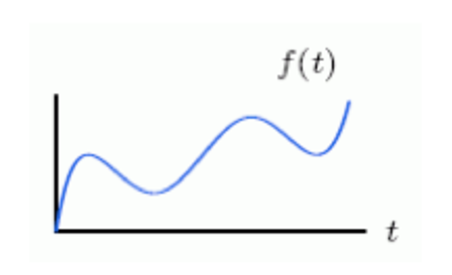
\includegraphics[width=5cm]{crit-n-inflection.pdf}
\begin{flushright}
  \begin{tikzpicture}
    \draw (0cm,-0.2cm) rectangle (5cm,1.2cm);
    \draw (0cm, 1.8cm) rectangle (5cm,3.2cm);
  \end{tikzpicture}
\end{flushright}
\newpage

%%%%%%%%%%%%%%%%%%%%%%%%%%%%%%%%%%%%% Page 4
\noindent{\large\bf MATH 122}\hfill{\large\bf Third Midterm.}\hfill{\large\bf
  Spring 2012}\hfill{\large\bf Page 4/5}\hrule

\bigskip
{\problem[10 pts] \em Use the first derivative for find all critical
  points and use the second derivative to find all inflection points.}
\begin{equation*}
f(x)=x^2-5x+6.
\end{equation*}
\vspace{2cm}
\begin{flushright}
  \begin{tikzpicture}
    \draw (0cm,-0.2cm) rectangle (5cm,1.2cm);
    \draw (0cm,1.8cm) rectangle (5cm,3.2cm);
  \end{tikzpicture}
\end{flushright}
\hrule
{\problem[10 pts] \em The marginal revenue and marginal cost of a
  company are $MR(q)=30$ and $MC(q)=0.03q^2-1.5q+36$ respectively,
  where $q$ is the number of items manufactured.  To increase profits,
  should the company increase or decrease production from each of the
  following levels?}
\begin{enumerate}
\item 25 items: The company should \framebox[3cm]{\raisebox{0.3cm}{}} production.
\vspace{3cm}
\item 50 items: The company should \framebox[3cm]{\raisebox{0.3cm}{}} production.
\vspace{3cm}
\item 80 items: The company should \framebox[3cm] {\raisebox{0.3cm}{}}
  production.
\end{enumerate}
\newpage

%%%%%%%%%%%%%%%%%%%%%%%%%%%%%%%%%%%%% Page 5
\noindent{\large\bf MATH 122}\hfill{\large\bf Third Midterm.}\hfill{\large\bf
  Spring 2012}\hfill{\large\bf Page 5/5}\hrule

\bigskip
{\problem[10 pts] \em Find the integral $\displaystyle{\int
    \frac{6x^5}{x^6+1} \, dx}$} 
\vspace{8cm}
\begin{flushright}
  \begin{tikzpicture}
    \draw (0cm,-0.2cm) rectangle (5cm,1.2cm);
  \end{tikzpicture}
\end{flushright}
{\problem[10 pts] \em Find the integral $\displaystyle{\int
    x^5(x^6+4)^2\, dx}$.}
\vspace{8cm}
\begin{flushright}
  \begin{tikzpicture}
    \draw (0cm,-0.2cm) rectangle (5cm,1.2cm);
  \end{tikzpicture}
\end{flushright}
\end{document}
